%; whizzy chapter
% -initex iniptex -latex platex -format platex -bibtex jbibtex -fmt fmt
% 以上 whizzytex を使用する場合の設定。


%     Tokyo Debian Meeting resources
%     Copyright (C) 2008 Junichi Uekawa
%     Copyright (C) 2008 Nobuhiro Iwamatsu

%     This program is free software; you can redistribute it and/or modify
%     it under the terms of the GNU General Public License as published by
%     the Free Software Foundation; either version 2 of the License, or
%     (at your option) any later version.

%     This program is distributed in the hope that it will be useful,
%     but WITHOUT ANY WARRANTY; without even the implied warranty of
%     MERCHANTABILITY or FITNESS FOR A PARTICULAR PURPOSE.  See the
%     GNU General Public License for more details.

%     You should have received a copy of the GNU General Public License
%     along with this program; if not, write to the Free Software
%     Foundation, Inc., 51 Franklin St, Fifth Floor, Boston, MA  02110-1301 USA

%  preview (shell-command (concat "evince " (replace-regexp-in-string "tex$" "pdf"(buffer-file-name)) "&"))
% 画像ファイルを処理するためにはebbを利用してboundingboxを作成。
%(shell-command "cd image200804; ebb *.png")

%%ここからヘッダ開始。

\documentclass[mingoth,a4paper]{jsarticle}
\usepackage{monthlyreport}
\usepackage[dvips]{xy}

% 日付を定義する、毎月変わります。
\newcommand{\debmtgyear}{2008}
\newcommand{\debmtgmonth}{7}
\newcommand{\debmtgdate}{19}
\newcommand{\debmtgnumber}{42}

\begin{document}

\begin{titlepage}
\thispagestyle{empty}

% タイトルページ:編集必要な部分は最初のマクロに飛ばすこと

\vspace*{-2cm}
第\debmtgnumber{}回 東京エリア Debian 勉強会資料

\hspace*{-2.4cm}
\includegraphics[width=210mm]{image200801/2008title.eps}\\
\hfill{}\debmtgyear{}年\debmtgmonth{}月\debmtgdate{}日

\end{titlepage}

\dancersection{Introduction}{上川 純一}
 
 今月のDebian勉強会へようこそ。これからDebianの世界にあしを踏み入れると
 いう方も、すでにどっぷりとつかっているという方も、月に一回Debianについ
 て語りませんか?

 Debian勉強会の目的は下記です。

\begin{itemize}
 \item \underline{Debian Developer} (開発者)の育成。
 \item 日本語での「\underline{開発に関する情報}」を整理してまとめ、アップデートする。
 \item \underline{場}の提供。
 \begin{itemize}
  \item 普段ばらばらな場所にいる人々が face-to-face で出会える場を提供
	する。
  \item Debian のためになることを語る場を提供する。
  \item Debianについて語る場を提供する。
 \end{itemize}
\end{itemize}		

 Debianの勉強会ということで究極的には参加者全員がDebian Packageをがりがり
 と作るスーパーハッカーになった姿を妄想しています。情報の共有・活用を通し
 て Debianの今後の能動的な展開への土台として、「場」としての空間を提供す
 るのが目的です。

以上を目的とした、2008 年アジェンダです:
\begin{enumerate}
 \item 新年会「気合を入れる」
 \item Open Source Conference Tokyo (3/1)
 \item データだけのパッケージを作成してみる、
       ライセンスの考え方 (David Smith)
 \item バイナリ一つのパッケージを作成してみる (吉田@板橋)\\
       バージョン管理ツールを使いDebianパッケージを管理する(git)\\
       アップストリームの扱い(svn/git/cvs)(岩松 信洋さん)
 \item バイナリの分けたパッケージの作成。(前田さん)\\
       バイナリの分け方の考え方、アップグレードなどの運用とか。
 \item パッケージ作成(dpatch/debhelperで作成するパッケージ)(小林儀匡さん)\\
       man の書き方(roff or docbook)(でんさん)
       OSC 2008 Hokkaido
 \item パッケージ作成(kernel patch、kernel module)(岩松 信洋)
       Debconf発表練習(上川さん)

 \item Debconf アルゼンチン、共有ライブラリパッケージ作成
       コミックマーケット74

 \item Open Source Conference Tokyo/Fall、
       デーモン系のパッケージの作成、latex、 emacs-lisp、フォントパッケージ
 \item パッケージの cross-compile の方法、amd64 上で i386 のパッケージと
       か、OSC-Fall報告会、Debconf報告会
 \item 国際化 po-debconf / po化 / DDTP
 \item 忘年会
\end{enumerate}


\newpage

\begin{minipage}[b]{0.2\hsize}
 \definecolor{titleback}{gray}{0.9}
 \colorbox{titleback}{\rotatebox{90}{\fontsize{80}{80} {\gt デビアン勉強会} }}
\end{minipage}
\begin{minipage}[b]{0.8\hsize}
\hrule
\vspace{2mm}
\hrule
\tableofcontents
\vspace{2mm}
\hrule
\end{minipage}

\dancersection{事前課題}{岩松 信洋}

今回の事前課題は
\begin{enumerate}
 \item Debian に取り込んでほしい Linux カーネルパッチ、Linux ドライバを教えてください。
 \item unstable でアップデートされなくて困ってる Debian パッケージ、BTS に登録されているバグのうち、早く直ってほしいバグを挙げてその理由を教えてください。
 \item {\bf ここで開催してくれないかなぁ} という勉強会の開催地をその理由と共に挙げてください (近いから、だけは却下!)。
\end{enumerate}
というものでした。
その課題に対して下記の内容を提出いただきました。

\subsection{鈴木 崇文 さん}
たいして需要もありそうでもなく、結構不安定だという話なので、個人的な趣味の問題ですが、vlookbackというカーネルモジュールが面白いので追加でインストールできるとうれしいです。vloopbackを使用すると、ビデオ出力に手を加えて仮想的なビデオ入力デバイスを通してループバックしたりでき、つまりdv入力をv4lに変換したり、uvcvideoデバイス(v4l2)をv4lに変換できたりしてustream.tvでのストリーミングが使えるようになったりします。
追加モジュールとしてdebパッケージで追加インストールできるのならば、今回の勉強会で学んで試しに自分用のパッケージを作成してみたいです。

\subsection{前田 耕平さん}

\begin{itemize}
\item Debian に取り込んでほしい Linux カーネルパッチ、Linux ドライバを教えてください。
Debianというよりは、LInux自体に対してなんですが、bcm4328がサポートされるとうれしいですね。Broadcomの製品概要を見るとLinuxはサポートOSにはなっているものの、Linux
Wirelessのサイトを見るとまだ対象外\footnote{http://ja.broadcom.com/collateral/pb/4328-PB02-R.pdf}
のようです。先日、Ndiswrapperを使ってようやくMacBook
Airで無線LANを利用できるようになったものの、黒MacBookに比べるとどうもIPアドレスの割り当てが不安定です(一度割り当てされると安定するんですが)。BBモバイルポイントでWEPで接続する分にはまったく問題無かったので、無線LANルータとの相性な気もしなくはないですが。\footnote{http://wireless.kernel.org/en/users/Drivers/b43\#unsupported}

Debianに、という観点では、特定のパッチやドライバというよりは、最新のパッチやドライバ、ソフトウェアのSidへの取り込みがもっと早ければなぁ、と思うことはあります。Upstreamに比べると遅くなるのは仕方が無いのですが、あまりにかけ離れてしまうと、自分でUpstreamの最新版を持ってきちゃえばいいかと、Debianパッケージは使わずに自分でビルドしてしまうので。

\item {\bf ここで開催してくれないかなぁ} という勉強会の開催地をその理由と共に挙げてください (近いから、だけは却下!)。

割と手頃な値段で借りられそうな候補を上げておきます。
\begin{itemize}
\item 晴海区民館
\url{http://www.city.chuo.lg.jp/sisetugaido/syukaisisetu/syukaisisetu17/}
インターネット接続環境はなし。プロジェクターも無いのがネックです。

\item ITS健保の会議室
半日借りられる、という点では割と安いです。プロジェクターは借りられます。
また、ITSの健保組合員がいないと借りられません。

\item 市ヶ谷会議室
\url{http://www.its-kenpo.or.jp/restaurant/itigaya_kaigisitu/index.html}
少人数(10人程度)の場合はまぁまぁかも。

\item 山王会議室
\url{http://www.its-kenpo.or.jp/restaurant/sannou_kaigisitu/index.html}
ある程度人数がいないとペイできません。(50人以上)

\item 大久保会議室
\url{http://www.its-kenpo.or.jp/restaurant/okubo_kaigisitu/index.html}
部屋の種類(定員)は一番多いです。

\end{itemize}
\end{itemize}

\subsection{やまねさん}
\begin{itemize}
\item BTS に登録されているバグのうち、早く直ってほしいバグを挙げてその理由を教えてください。

最近はバグウォッチしてないのでなんともむずかしいですが、自分が登録してる
ITP バグをクローズしたいなーとは日々思っています。思ってるだけで何もして
ないんですが。あとは l10n な ja.po は登録して1年とか放置されると悲しい
気分になるので早めにお願いしたい所です(最近はi18nなNMUでfixされますが)。

つーかね、動かねーとか何か変とかいうんだったら、BTS に追加情報だせよゴルァ!
とか思ったりしたりしなかったりする今日この頃。
\end{itemize}

\subsection{あけどさん}
\begin{itemize}
\item unstable でアップデートされなくて困ってる Debian パッケージ、BTSに登録されているバグのうち、早く直ってほしいバグを挙げてその理由を教えてください。

net-toolsパッケージのいろんなバグ
特にnetstatコマンドのIPv6アドレスが切り落とされるバグは
lenny以降での対応が IPv4 アドレスを表示する形になっていて
ぱっと見ただけで如何にもダメな印象になってしまうので
upstreamを含めて何とかして欲しいところです。

ちなみに他の某ディストリビューションでは
IPv6アドレスが正常に表示されるようになっていて
とても悲しかったりします。

どうやったらプロパーな状況になるんでしょうか?
\end{itemize}

\subsection{伊藤 弘和さん}
\begin{itemize}
\item unstable でアップデートされなくて困ってる Debian パッケージ、BTSに登録されているバグのうち、早く直ってほしいバグを挙げてその理由を教えてください。

バグというよりは、open-vm-toolsパッケージの修正が一段落ついて欲しいなと思っております。
熱い状態ということもありますが自分も常用している物こそ、貢献できるようになりたいとパッケージの熟成をウォッチしています。
\end{itemize}

\subsection{大波 誠さん}
\begin{itemize}
\item Debian に取り込んでほしい Linux カーネルパッチ、Linux ドライバを教えてください。

正直に申し上げます。パッと思いつくものがありませんでした。ただ、この機会
に「Linux ドライバ」とか「debian ドライバ」とかでぐぐってみました。そした
らThe Linux Foundationがデバイスドライバのオープンソース化を声明として発表
していたり グラフィックボードのドライバなどのプロプライエタリなソフトウェ
アに関する問題が載っていたりして勉強になりました。
前田 耕平さんから勉強会を紹介していただきました。
初参加させていただきます。
\end{itemize}

\subsection{市川 憲人さん}
\begin{itemize}
\item Debianに取り込んで欲しいLinuxカーネルパッチ

個人的な事情なのですが、自宅サーバがMacBookでそのネット 
ワークインターフェイスが
Marvell Yukon 88E805xで、kernel標準のsky2ドライバ 
はやや挙動が怪しいので、
Marvell提供のドライバをdebianのパッケージ化してあると便 
利です。
自分の技術力ではmake bzImageすら通らなかったので
どなたか技術力のある方がパッケージ化して下さると大変嬉しいです。
\end{itemize}

\subsection{本庄さん}
\begin{itemize}
\item Debian に取り込んでほしい Linux カーネルパッチ、Linux ドライバを教えてください。

特に思いつかないです。

\item unstable でアップデートされなくて困ってる Debian パッケージ、BTS に登録されているバグのうち、早く直ってほしいバグを挙げてその理由を教えてください。

アップデートされなくて困っているというわけではありませんが、最近
webminを使いたいと思うことがあり、ちょっと残念でした。


\item {\bf ここで開催してくれないかなぁ} という勉強会の開催地をその理由と共に挙げてください (近いから、だけは却下!)。

以前にも話に上がっていた、温泉宿はどうでしょう。夜を徹して語り合
う先になにかが見えるかもしれません。
\end{itemize}

\subsection{濱野さん}
\begin{itemize}
\item Debian に取り込んでほしい Linux カーネルパッチ、Linux ドライバを教えてください。

netfilter の P-O-M patch に含まれる ipset というモジュールを使用してい
ます。なかなか mainstream に入ってくれない様なので package で用意してお
くと便利かな、と思いました。

もうひとつ La Fonera のイメージを触るのに squashfs もあると嬉しいかな、
mksquashfs というユーザランンドツールでこと足りてたりもするのですが\tt\symbol{94}\tt\symbol{94};
\end{itemize}

\subsection{青木 修}
まあ、かなり利用者の増えているSCIMですがパケージングに参加されている人が
すくないので、なかなかアップデートが追いつきません。

メインのMINGさんは忙しいので、協力してくれるかたいません?私は単なる
UPLOADERで技術的にこれは難しいので、いい人探しています。

あー、開催場所ですが、東工大の長津田キャンパスなどだれか学生さんがいそう
なのになぜないのかなーといつも思っています。

\subsection{藤沢 理聡 さん}
\begin{itemize}
\item {\bf ここで開催してくれないかなぁ} という勉強会の開催地とその理由

開催地:学校(高校・大学など)
理由:
一言で言うと、学生に興味を持って欲しいからです。
Debianに触れるのに年齢は関係ないと思うけれど、
若いうちにDebianに触れるのも悪くないと思います。
学校という場所や学生という立場では、
今のところLinuxのようなフリーなOSに触れる機会は
多くないのが残念です(社会に出ても触れる機会は多くないけど)。
とにかく、まだ知らない人が興味を持ってくれそうな、
そういう場所で開催するのもいいんじゃないかな、と思いました。
\end{itemize}

\subsection{岩松 信洋}
\begin{itemize}
\item Debian に取り込んでほしい Linux カーネルパッチ、Linux ドライバを教えてください。

今回の資料作成のついでに作りました。内容は発表を参照。

\item unstable でアップデートされなくて困ってる Debian パッケージ、BTS に登録されているバグのうち、早く直ってほしいバグを挙げてその理由を教えてください。

kernel-package 関係のバグなど。メンテナ(Manoj)サボリ気味ですね。困りましたね。
libflash の不具合が直ってないのをなんとかしてほしい。

\item {\bf ここで開催してくれないかなぁ} という勉強会の開催地をその理由と共に挙げてください (近いから、だけは却下!)。

先日、東京電機大学さんに行って、コラボできないか相談してきました。学生さんに興味を持たせるにはどうしたらいいですかね。
あとは温泉を8月に企画中です。

\end{itemize}

%%% trivia quiz
\dancersection{Debian Trivia Quiz}{小林 儀匡}

ところで、みなさん Debian 関連の話題においついていますか?Debian関連の話
題はメーリングリストをよんでいると追跡できます。ただよんでいるだけではは
りあいがないので、理解度のテストをします。特に一人だけでは意味がわからな
いところもあるかも知れません。みんなで一緒に読んでみましょう。

今回の出題範囲は\url{debian-devel-announce@lists.debian.org} に投稿された
内容とDebian Project Newsからです。
% 出題範囲: http://lists.debian.org/debian-devel-announce/2008/06/msg00004.html 〜 http://lists.debian.org/debian-devel-announce/2008/07/msg00004.html
\begin{multicols}{2}
 \subsection{debian-devel-announce}
 \url{debian-devel-announce@lists.debian.org}への投稿内容からです。
 
 \santaku
 {Perl 5.10のバグでどのような問題が発生した?}
 {RubyとPythonで書かれたアプリケーションやライブラリがインストールできない}
 {インストールされたファイルのパーミッションが0777になる}
 {特定の名前のファイルがインストールできない}
 {B}% File::Path::rmtreeがツリー削除前にパーミッションを0777にし、それがsymlinkのリンク元にも伝播するようになっていたのが原因。postinstで呼び出されるdebsignがツリーのsymlinkを作成してハッシュを計算した後、この関数を使ってsymlinkを削除しているので、インストール後にファイルのパーミッションが書き換えられる問題に発展した
 
 \santaku
 {Debianプロジェクト内のチームに関する調査で判明した「予想外のチーム」でないものは?}% 調査はDPLのSteve McIntyreが行っている
 {実際に動いているのは1人だけというチーム}
 {誰が作業するか毎回じゃんけんで決めているチーム}
 {お願いやありがとうではなく脅迫で動いているチーム}
 {B}
 
 \santaku
 {wxwidgets2.8がアップロードされたが、長いことwxwidgets2.6の時代が続いていた。その理由は?}
 {パッケージメンテナが保守的で、2.8の使用に対して非積極的だった}
 {アップロードしたところでどうせ誰も使ってくれないとパッケージメンテナが思った}
 {パッケージメンテナが多忙で作業時間がとれなかった}
 {A}% lennyでは2.6をデフォルトとし、2.6で動かないものだけ2.8を使ってほしい、とのこと
 
 \santaku
 {Frans Popの辞任によって、新たな執筆者が求められるようになったものとは?}
 {リリースノート}
 {Debian Project Blog}% Debian Project公式のblog
 {DEB NOTE}% 名前が書かれた開発者を強制的にコミュニティから追い出すノート
 {A}
 
 \subsection{Debian Project News 2008年05号}
 \url{http://www.debian.org/News/weekly/2008/05/}
 にある6月23日版です。
 
 \santaku
 {debian/rulesのget-orig-sourceターゲットは何を記述するためのものか?}
 {「オリジ○弁当」で弁当にソースをつけてもらう方法}
 {upstreamからネットワーク経由でソースコードを取得して現在のソースコードと置き換える方法}
 {upstreamからネットワーク経由で最新の.orig.tar.gzファイルを取得する方法}
 {C}% あまり書かれることのないターゲットだが、skkdicではCVS経由で取得するよう設定している
 
 \santaku
 {リリースゴールに関するPeter Eisentrautの意見は?}
 {リリースゴールなんて所詮一部の開発者の楽しみに過ぎない}
 {Debianの機能の実装に関するリリースゴールはリリース後にポリシーへと変えるべきだ}
 {リリースなんて飾りです。偉い人にはそれがわからんのですよ}
 {B}
 
 \santaku
 {William Pitcockが削除を提案したブートローダパッケージは?}
 {grub}
 {lilo}
 {yaboot}
 {B}% 簡単には直せないgraveなバグがある
 
 \santaku
 {Debian weatherとはどんなサービスか?}
 {特定アーキテクチャのアーカイブの状態を要約して表示する}% その表示に天気の記号を使用している
 {Debian関連ホストが置かれている世界各地の天気を表示する}% worldwideで働いているという意識を高める
 {メーリングリストの流量から世界各地の天気を推測して表示する}% この地域からのメールが多いからこの地域は雨だな、とか
 {A}
 
 \subsection{Debian Project News 2008年06号}
 \url{http://www.debian.org/News/weekly/2008/06/}
 にある7月7日版です。
 
 \santaku
 {Debian 15周年はいつか?}
 {次回の東京エリアDebian勉強会開催予定日である8月16日}
 {本日7月19日}
 {泣く子も黙る7月9日}
 {A}
 
 \santaku
 {Debianのメニュー (.menuファイル) とデスクトップ環境のメニュー (.desktopファイル) に関する議論はどのような結論に落ち着いたか?}
 {freedesktop.orgの.desktopファイルをDebianに合うよう拡張して使っていこう}
 {freedesktop.orgの.desktopファイルには不便な点があるので、働きかけて修正してもらおう}
 {freedesktop.orgの.desktopファイルは使えないのでDebianの.menuファイルを使わせよう}
 {A}% .desktopメニューはユーザビリティを目的とするもので単一階層 (サブカテゴリなし) なのに対し、Debianのメニューは完全性を目的とするもので階層を深く掘っている。ちなみに.menuに比べて.desktopのほうがいいという人はかなり多そう
 
 \santaku
 {6月末に初めて誕生したDebian開発者同士の夫婦とは?}
 {Junichi UekawaとKenshi Muto}
 {Meike ReichleとAlexander Schmehl}
 {Debra MurdockとIan Murdock}% 実はDebraさんがDDになり今更ながら結婚、とか
 {B}
 
 \santaku
 {結婚した二人について述べた以下の事項のうち、正しいものは?}
 {最初の贈り物: DebConf5の土産}% 具体的にはDebConf5のTシャツとフィンランドのチョコレート
 {秘密の愛の交換手段: wiki.debian.org}% planet.d.oで交換していたら誰かに書き換えられた
 {婚約の公式発表手段: lists.debian.org}% planet.d.oで発表したら名前を書き換えられた
 {A}

\end{multicols}
\dancersection{最近のDebian関連のミーティング報告}{岩松 信洋}
\subsection{東京エリアDebian勉強会41回目報告}
6月の第41回東京エリアDebian勉強会を実施しました。 今回の参加者は あけどさん、前田さん、小林儀匡さん、吉田@板橋さん、山本 浩之さん、 山本琢さん、藤沢理聡さん、日比野 啓さん、鈴木 邦男さん、岩松の10人でした。

\begin{itemize}
    \item まず最初に最近のミーティングの報告を行いました。
    \item 今回のクイズは岩松が出題しました。全問正解者はいませんでした。似たような答えが多く、回答者は困っていました。
    \item 事前課題を紹介しました。 AIXのログシステムと提供されている errpt コマンドがかなりいけているようです。実際に実機を触ってどんな感じなのか見てみたいです。あと、hinemos の話が出ました。Debianで使いたい方が多いようですが、Java で実装されており、要求するマシンスペックも高いため、パッケージングとテストの道のりは激しく遠い気がしました。
    \item 2008年のテーマはDEBパッケージの開発・管理に関連した内容ですが、 4回目のテーマとして小林さんがdebhelperを使ったパッケージング方法について紹介しました。debhelper を使わないパッケージング方法から、debhelper を使った方法、cdbs を使った方法をいう流れで話してくれたので、debhelperとcdbsのありがたさが分かりました。
    \item 最近の kFreeBSD, nexenta, Hurd, SuperH, eeepc について紹介して終了しました。
    \item 隠し球だった山本さんの Hurd ユーザーを増やす会の発表ができませんでした。
    \item 今回も勉強会の間違えてしまった人がおられました。開催場所は毎回チェックするようにしましょう。
    \item 勉強会のあと、居酒屋さつきで宴会をしました。Debian ぐるぐるカッティングステッカーを販売してみたところ、なかなかの好評ぶりでした。さっそくPCに貼っている人もおり、大満足のようです。ステッカーが欲しい人は私に連絡をください。 
\end{itemize}

% (query-replace-regexp "<.*?>" "")
% (query-replace-regexp "^[	 ]\+" "")


\subsection{eeePC Developers Conference day 1}

経済部工業局。
登録したら無料で参加できるカンファレンス。
講演者が全員スーツをきていますが、来場している方々は普段着です。
カメラのフラッシュの量からは注目度が伺えます。
携帯電話の着信音がなりほうだいです。

開始のオープニングは多少おくれましたがほぼ満員で開始しました。
後半になると半分くらいの埋まり方になりました。

みなさまeeePCでプレゼンしていますが、
プロジェクターが同期とれていない感じで、全体がうつっていません。

外は暑く、会場が寒いのだけど、みんななれているものでジャンパー着てます。

5月8日に1日目が開催されました。

\begin{tabular}{|c|p{18em}|c|}
09:00 ~ 09:30 & 	 Register & \\
09:30 ~ 09:45 &	Opening Remarks & \\
09:45 ~ 10:20 &	Keynote Speech Keynote Speech -- EeePC Software Platform Business Model &	ASUS | Ellis Wang\\
10:20 ~ 10:50 &	EeePC Application Demo Show &	ASUS  Patrick Chou\\
10:50 ~ 11:00 &	Tea Break &\\
11:00 ~ 12:20 &	EeePC SDK Announcement and Demo &	ASUS\\
12:20 ~ 13:40 &	Lunch &\\
13:40 ~ 14:30 &	The rule of game to stand on the shoulders of giant 	&Florence T.M. Ko, OSSF\\
14:30 ~ 15:10 &	Developing with pyGTK in EeePC 	&TsungWei Hu, OSSF\\
15:10 ~ 15:30 &	Tea Break &\\
15:30 ~ 16:10 &	Developing with pyQT in EeePC 	&Gary Lee\\
16:10 ~ 16:50 &	Firefox Platform Application Programming 	&Thinker\\
16:50 ~ 17:30 &	Google Gears Programming 	&Tzeng Chien-Ming\\
17:30 ~ 17:40 &	Software Vendor Panel Discussion 	&ASUS\\
\end{tabular}


\subsubsection{開会のご挨拶}

eeePC SDK の発表

Open Source Development

\subsubsection{開会のご挨拶2}

何かの話、まったくわからず。

\subsubsection{Announcement of eeePC SDK, Dev tools and Community}

ASUSのEllis Wang氏が発表しました。
eeePCでプレゼンしています。
オープンソースのデベロッパーの人たちにできるだけ参加してほしいという気持
ちが伝わってきます。
英語のプレゼンで、中国語で発表しています。

最初に開会の挨拶をしたえらいひとになぜかeeePCを贈呈しています。

Linux で、コミュニティーについてなんたら。

ISVとコミュニティー

SDKの話。

ASUSとeeePCのソースコードが
ツールダウンロードできるよね。

オープンソースコミュニティーがeeePCを支援している。

Linux にかぎらず、Debian, KDE などがある。

MicrosoftのUIに比べて、UIの変更が簡単と言っているような気がする。

Linux の素晴らしさについて。
EeePC:

\begin{itemize}
 \item easy -- to learn, work and play
 \item excellent -- on the go
 \item excellent -- internet experience
\end{itemize}

インテグレーションすることの大切さ。
contribution を行う。

汎用のツールのソースを組み合わせて作り上げる。

オープンソースは共有することが大切であり。
IPの話。
[share]

warranty の話?

reuseの話。


EeePC SDKとは?

マニュアルの目次を画面にうつす。
EeePCのパッケージはDebianパッケージだよ。

パッケージのテストは?VMwareをつかおう。

eeePCは開発者・ASUS・ユーザ・CCデジタルコンテントをつなぐためのブリッジだ。

無線とかCPUとかカーネルとかはASUSがやるだろ?

GPLだろ、とか。

Debianのパッケージとかを提供する。

バーチカルでNo1を目指す。
テレコムと教育目的に。

partner のレベルがある。

システムとOSのパートナーは一番少ないがインテグレーションの度合いが高い。

SDK作ったのでオープンソースデベロッパーたちにデベロップメントコミュニティー
をつくることができるだろ?
コマーシャルベンダーもツールが充実していて満足するにちがいない。
オープンソースの技術者もよく知っている技術でうれしいに違いない。

Eclipse と Qt4 の開発ツールキットがはいっているぜ。

開発プロセスの
Phaseは二種類ある。
実機とVMwareだ。
フェーズイーとフェーズアル。


テストの小技。
画面サイズとか全部試しておくのがよいです。

デスクトップと比べると一部違います。
ASUS desktopで、ユーザアカウントが一つしかないよ。
また、initはミニマルです。

howto 

画面小さい。
Flashは10万回書き込むと wear out するのでできるだけ書き込みしない。

eeePCアプリケーションの移植は簡単よ。
Javaも動く。PicasaはWineで動いている。
(Linuxの説明をしている気がする。)

Adobe flash はサポートするけどAIRはダメだね(?)。


と、終わったら人が騒然としはじめた。
休憩時間開始。スナックとコーヒーが提供されました。

\subsubsection{教育用のアプリケーション?}

株式取引ツール

発音の出る辞書

カラオケみたいな、音楽が流れながら歌詞と訳語の出るツール。

ASUS MeBook

MeReader MeSong


本を買うことができる。

ラップ風の中国語会話。IQChinese。
PinYinの勉強させてくれる。


音声制御のツール。Skypeを声で起動できる?

一ページめくると音声で指示を出してプレゼンを制御している。

\subsection{Introduction to eeePC SDK}

Chih Wei Huang

赤ちゃんでもつかえるくらいシンプルだよ、
と赤ちゃんの写真を見せてice-break。

eeePC900 は2008年4月、8.9'' シリーズとして登場。

eeePCはDebianベースです。
オープンソースですよ。

Xandros open circulation edition というのをつかってます。
開発環境はEclipse です。

Qt4は今はNokiaのTrolltechが開発。


標準の.debパッケージを使っている。
SDKとして、debian policy manual, new maintainer guideとかが紹介。
エキスパートがたくさんいるよ、と。

デスクトップにアイコンを追加する方法は簡単だよ。
XMLファイルを作成すればよい。

\url{http://sourceforge.net/projects/eeecommunity/}
にVMware のイメージはあるから見てね。
ISOをvmware-convert コマンドで変換したら利用できるよ。
eeePC 701 のイメージなどがある。

i18n/l10nは、Qt と gettext があるよ。
Qt は tr().
lupdateとか使う。
gettextは \verb!_()!で。


EclipseのQt用の開発ツールがあるよ。
Qt Designer が Eclipse内部で動作します。


\subsubsection{The rule of game to stand on the shoulders of giant}

GPLの呪縛を回避する方法について。

FOSSの裁判案件の紹介。

Busybox 裁判など。

Creative Commons のすすめとか。

質問は、GPL の継承を避免する方法について。
dynamic linker と static link の話をしていたような気がする。

\subsubsection{Developing with pyGTK in EeePC}

??
Open Source Software Foundry Introduction かも?

自由とは。

OSSFの話

Pythonを使うことについて。
python の文法について。インデント重要とか

Gtk とか。

\subsubsection{Developing with pyQT in EeePC}

PyQtの使用方法についての紹介。

\subsubsection{Firefox Platform Application Programming}

ハッカー然とした「thinker」による firefox プラットフォームアプリケーションプログラミング
の紹介。

「OK」としか表示しない mozilla アプリケーションの例の紹介。XUL。

時間オーバーだということで途中できりあげられてしまいました。

\subsubsection{Google Gears Programming}

Google Gears を利用して開発する方法について紹介しています。

\subsection{eeePC Developers Conference day 2}

5月9日に2日目が開催されました。

当初の発表されていた予定から大幅に変更されて実施されました。

\begin{tabular}{|c|p{18em}|c|}
09:00 ~ 09:30 &	Register & \\
09:30 ~ 10:00 &	Eclipse,Gambas,Lazarus Development Environment Introduction& 	ASUS \& III Free Software Team\\
10:00 ~ 10:50 &	Adobe Air Platform Programming 	&Anistar Sung\\
10:50 ~ 11:00 &	Tea Break& \\
11:00 ~ 12:00 &	Eee PC Hacker Show 	&ASUS SAM\\
12:00 ~ 13:30 &	Lunch & \\
13:30 ~ 14:00 &	EeePC HotKey、WebCAM、Audio Control 	&ASUS \& III Free Software Team\\
14:00 ~ 14:15 &	Introduction of Open Source Development Resource and Discussion Forum &	III Free Software Team\\
14:15 ~ 14:30 &	Open Source Software Foundry Introduction 	&Tim Wu, OSSF\\
14:30 ~ 15:30 &	Debian Project and the Development Process, and how to co-work with it 	&Junichi Uekawa\\
15:30 ~ 15:40 &	Q \& A 	& \\
15:40 ~ 16:00 &	Tea Break & \\
16:00 ~ 17:00 &	Linux Driver Project 	&Brandon D. Philips\\
17:00 ~ 17:10 &	Q \& A 	& \\
\end{tabular}


\subsubsection{GTK?}

10時ころについたら何か違う人が話をしていた。




\subsubsection{Eclipse,Gambas,Lazarus Development Environment
   Introduction}

「IDEAS III」

MonoDevelop

Lazarus は PASCALのツール

なんか途中かなと思っていたら話が終わっていた。

\subsubsection{LXDEの紹介}

pcman による LXDEの紹介?


起動がすごく高速、リソースも全然
使わないというデモ。
ファイルマネージャをクリックしまくって起動してもスムーズだぜ!

計算機とかも便利!

タスクバーとか、パネルとか。

\subsubsection{Deb?}

\subsubsection{Array 30入力メソッド}

新しい input method を作った。
アレーベースの方法。

GCIN OXIMという古いもの、SCIMに。
現在SCIMは日本語とコリアンの入力に必須。

で、頑張っていろいろと入力してみる。

\subsubsection{EeePC HotKey}

ホットキーのプログラムの書き方について紹介。
GDKでhkのコールバックがあります、という紹介。

\subsubsection{eeePC audio, webcam}

オーディオはALSAです、Wikiを見てください。

webcam の制御は、unicapGTKでやります。
ucilはビデオに文字とかを載せるためのAPIです。

unicapGTKの開発の話。

\subsubsection{Open Source Software Foundry Introduction}

フリーソフトウェアを支援する環境の紹介。

フリーソフトウェアを工業的統合を経たら製品になる素材と位置づけて推進して
いく。

\subsubsection{Adobe Air Platform Programming}

AIRプラットフォームの紹介。RIAのためのAIR。

\subsection{OSC 2008 Hokkaido}
OSC 2008 Hokkaido に Gitの話をしてください、と呼ばれたのでDebian勉強会として行ってきました。
最近流行っている SCM Git ってどうよ?というネタで、Gitの魅力と簡単な使い方についてお話させてもらいました。
15人の登録でしたが、実際は30人ぐらいの参加でした。45分では基本的なところしか話せないので、
うまくGitの良さを使えることができなかったかもしれません。けど、基本的な使い方は分かるように説明したつもりなので、
感想とかあれば教えてください。RubySapporoの方に ustream と録画をしてもらいましたが、うまく撮れてなかったとのこと。
残念。北海道の方やRubyの高橋さんとお話する機会があり、勉強会をどのように盛り上げていくのか、意見交換をしました。
が、酔っ払っていたのであまり覚えていないです。

\dancersection{Linux カーネルパッチ の Debian パッケージ作成}{岩松 信洋}
\label{sec:kpatch}
\index{kpatch}

\subsection{はじめに}
テスト段階の機能が Linux カーネルへのパッチとして公開されている場合がありますが、
これらの パッチを Debian で利用したい場合には、Debian で配布している カーネルパッケージや vanilla カーネルに
パッチを当ててパッケージ化されている方も多いのではないでしょうか。
Debian の特徴の一つしてパッケージ管理が挙げられますが、実は Linux カーネルパッチも Debian パッケージとして管理することができ、
既にいくつかのパッケージが利用可能になっています。
また、この Linux カーネルパッチパッケージを作成するためのサポートパッケージ {\bf dh-kpatches} 
が提供されており、このパッケージを利用することよりパッチ用パッケージの作成や、
カーネルへのパッチ適用およびコンパイルが可能になっています。
今回は Evgeniy Polyakov(えぶじぇにー ぽるやこふ)が作成している
新しい Network Filesystem POHMELFS\footnote{\url{http://tservice.net.ru/~s0mbre/old/?section=projects&item=pohmelfs}}
を題材にして、Linux カーネル向けパッチのパッケージ作成方法とテスト方法について説明します。

\subsection{Linux カーネルパッチ の Debian パッケージの仕組み}
Linux カーネルパッチパッケージは、カーネルパッチと パッチをコントロールするためのファイル kpatches を提供します(図\ref{fig:kpatch0})。
このファイルでは、アーキテクチャ、カーネルバージョンの指定が可能になっています。
そして、パッケージ作成時に kpatches ファイルからpatch/unpatch 時に使用される パッチコントロールスクリプトが生成されます。
パッケージをインストールすると、/usr/src/kenel-patches ディレクトリに各ファイルが展開されます。
Debian カーネルパッケージを作成するためのコマンド make-kpkg の --added-patches オプションで 指定された
パッチパッケージ名を このディレクトリから検索し、パッチを適用してから、カーネルをコンパイルします。
\begin{figure}[h]
 \begin{center}
  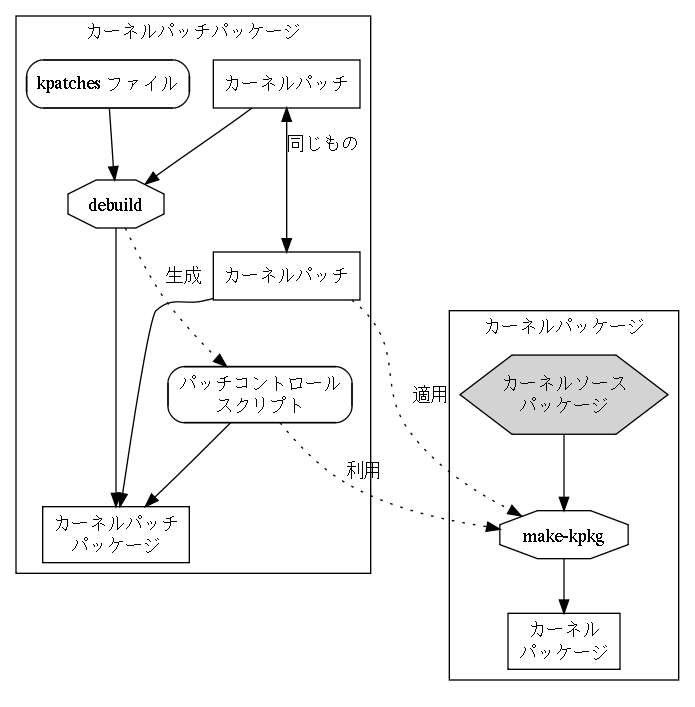
\includegraphics[width=0.8\hsize]{image200807/kpatch0.png}
 \end{center}
 \caption{Linux カーネルパッチ の Debian パッケージの仕組み}
 \label{fig:kpatch0}
\end{figure}

\subsection{パッケージ作成前の準備}

\subsubsection{dh-kpatches パッケージのインストール}
make-kpkg が利用できる Linux カーネルパッチパッケージを作成するには、dh-kpatches パッケージが必要です。
dh-kpatches を使って、パッケージ化
を行うことにより、kenrel-package で提供されている make-kpkg コマンドでカーネルパッチパッケージで提供している
パッチを適用した Linux カーネルパッケージが作成できるようになります。
パッケージ作成サポート用として、dh-make をインストールしておくと良いでしょう。dh-make を使うことによって、パッケージの
雛形を容易に作成することができます。
\begin{commandline}
$ sudo apt-get update
$ sudo apt-get install dh-kpatches dh-make build-essential
\end{commandline}

\subsubsection{パッチの用意}
まず、カーネル向けのパッチを作成する必要があります。開発者によっては、既にパッチがカーネルバージョン毎に用意されている事もありますが、
最近では、Linus のツリーに容易に追従できるように、Gitを使ってソースコードが管理されている場合が多いです。
POHMELFS でも ソースコードは Git で管理されており、安定版のカーネル(この原稿を書いている時点では、Linux 2.6.25)に常に追従されています。
この差分を取得するには、Git リポジトリを取得し、git diff コマンド等で取り出せばよいでしょう。

\begin{commandline}
$ git clone http://tservice.net.ru/~s0mbre/archive/pohmelfs/pohmelfs.git
Initialized empty Git repository in /tmp/pohmelfs/.git/
got 37e1b82c0535386cf09b3821dff5e8cb5f9e26b4
walk 37e1b82c0535386cf09b3821dff5e8cb5f9e26b4
<snip>
$ cd pohmelfs
$ git tag
<snip>
v2.6.24-rc8
v2.6.25
v2.6.25-rc1
v2.6.25-rc2
<snip>
$ git diff v2.6.25 > ~/pohmelfs.diff
\end{commandline}

\subsubsection{ディレクトリの作成}

パッチが作成できたら、パッケージ作成用のディレクトリを作成し、その中にパッチファイルをコピーします。
ディレクトリ名は Debianのポリシーに合わせたもの(ソフトウェアまたは機能名-バージョン)にしておき、パッチファイル名は
パッチ機能名-カーネルバージョン にしておきます。これは、このようなファイル名を dh-kpatches が要求するためです。

\begin{commandline}
$ mkdir linux-patch-pohmelfs-20080707
$ cd linux-patch-pohmelfs-20080707
$ cp ../pohmelfs.diff pohmelfs-2.6.x
\end{commandline}

\subsection{dh\_make を使った雛形の作成}
パッケージ作成の準備ができたら、 dh\_make コマンドを使って雛形を作成します。
dh\_make にはカーネルパッチ用のサポートはないので、singleバイナリの雛形を作成する
オプションを指定して、作成します。-r オプションは orig.tar.gz ファイルを作成し、-s オプションは
シングルバイナリ用の雛形を出力します。
\begin{commandline}
$ dh_make -r -s
Maintainer name : Nobuhiro Iwamatsu
Email-Address   : iwamatsu@nigauri.org 
Date            : Mon, 07 Jul 2008 01:00:33 +0900
Package Name    : linux-patch-pohmelfs
Version         : 20080707
License         : blank
Using dpatch    : no
Type of Package : Single
Hit <enter> to confirm: 
Currently there is no top level Makefile. This may require additional tuning.
Done. Please edit the files in the debian/ subdirectory now. You should also
check that the linux-patch-pohmelfs Makefiles install into $DESTDIR and not in / . 
\end{commandline}

\subsection{debianディレクトリ内の変更}
dh\_make コマンドで カーネルパッチを Debian パッケージにするための雛形が作成できました。
これを元に内容を変更していきます。

\subsubsection{サンプルスクリプト等の削除}
dh\_make で作成されるサンプルスクリプトは必要ないので全て削除します。
また、 dirs ファイルや doc ファイルも必要ないため削除します。
\begin{commandline}
$ rm -rf ./debian/*.ex ./debian/*.EX ./debian/docs ./debian/dirs
\end{commandline}

\subsubsection{debian/copyright の修正}
パッチの情報に合わせて、debiab/copyright の修正を行います。
pohmelfs の場合は以下のように修正します。

\begin{commandline}
This package was debianized by Nobuhiro Iwamatsu <iwamatsu@nigauri.org> on
Mon, 07 Jul 2008 01:00:33 +0900.

It was downloaded from
        http://tservice.net.ru/~s0mbre/archive/pohmelfs/pohmelfs.git
This is Git repository. I made the difference of the latest committing a
patch from v2.6.25 tag.

Upstream Author(s):

    Evgeniy Polyakov <johnpol@2ka.mipt.ru>

Copyright:

    Copyright (C) 2008 Evgeniy Polyakov <johnpol@2ka.mipt.ru>

License:

 GPLv2

The Debian packaging is (C) 2008, Nobuhiro Iwamatsu <iwamatsu@nigauri.org> and
is licensed under the GPL, see `/usr/share/common-licenses/GPL'.

# Please also look if there are files or directories which have a
# different copyright/license attached and list them here.

\end{commandline}

\subsubsection{debian/README.Debian の修正}
debian/README.Debian ファイルに Debian で使うための HowToなどを書いておきましょう。
サポートしているカーネルバージョンや、カーネルイメージの作成方法などを書いておくのが一般的
なようです。

\begin{commandline}
linux-patch-pohmelfs for Debian
-------------------------------

This patch is pohmelfs support patch for Debian Linux kernel. 
You can try with linux-source-2.6.25 package. 

- How to use
  $ sudo apt-get install linux-source-2.6.25 libncurses-dev kernel-package
  $ cd /usr/src ; tar -xjf linux-source-2.6.25.tar.bz2 ; cd linux-source-2.6.25
  $ make-kpkg clean
  $ cp /boot/config-2.6.25-2-686 .config
  $ make menuconfig
  $ make-kpkg --rootcmd fakeroot --append-to-version -pohmelfs --revision 0.1 -added_patches=pohmelfs kernel-image

 -- Nobuhiro Iwamatsu <iwamatsu@nigauri.org>  Mon, 07 Jul 2008 01:00:33 +0900

\end{commandline}

\subsubsection{debian/control の修正}
次に debian/control ファイルを修正します。
注目すべきところは、作成されるパッケージで指定してある、{\bf Depends: \$\{kpatch:Depends\}}です。
ここで kpatch:Depends を指定することによって、カーネルパッチパッケージを使った
カーネル作成に必要な依存パッケージを置き換えてくれます。
また、ソースパッケージの {\bf Build-Depends} に {\bf dh-kpatches パッケージ} を追加する事を忘れないようにしましょう。

\begin{commandline}
Source: linux-patch-pohmelfs
Section: devel
Priority: extra
Maintainer: Nobuhiro Iwamatsu <iwamatsu@nigauri.org>
Build-Depends: debhelper (>= 6), dh-kpatches
Standards-Version: 3.8.0.1
Homepage: http://tservice.net.ru/~s0mbre/old/?section=projects&item=pohmelfs

Package: linux-patch-pohmelfs
Architecture: all
Depends: ${kpatch:Depends}
Description: POHMELFS kernel patch
 POHMELFS stands for Parallel Optimized Host Message Exchange Layered File System.
 Development status can be tracked in filesystem section.
 This is a high performance network filesystem with local coherent cache of data
 and metadata.
 Its main goal is distributed parallel processing of data. Network filesystem is a
 client transport.
 POHMELFS protocol was proven to be superior to NFS in lots (if not all, then it
 is in a roadmap) operations.
\end{commandline}

\subsubsection{debian/changelog の修正}
dch コマンドを使って debian/changelog ファイルを修正します。
\begin{commandline}
$ dch
linux-patch-pohmelfs (20080707-1) unstable; urgency=low

  * Initial release                                          

 -- Nobuhiro Iwamatsu <iwamatsu@nigauri.org>  Mon, 07 Jul 2008 01:25:37 +090
\end{commandline}

\subsubsection{kpatches ファイル}

どのパッケージ内に収録されているパッチをどのカーネルバージョンに当てればいいのかなどの
コントロールするためのファイル kpatches を用意する必要があります。
このファイルは以下のようなフォーマットになっており、
カーネルバージョン毎に Patch-file と Kernel-version の項目を追加する必要があります。
また、このファイルを {\bf パッケージ名.kpatches} として 名前を変更する必要があります。

\begin{commandline}
Patch-name: POHMELFS patch
Patch-id: pohmelfs <-- make-kpkg の --added-patches で指定するパッチ名 
Architecture: all <-- サポートするアーキテクチャ
Path-strip-level: 1

Patch-file: pohmelfs-2.6.x <-- パッチファイル名
Kernel-version: 2.6.25 <-- パッチがサポートするカーネルバージョン
\end{commandline}

\subsubsection{debian/rules ファイルの修正}
debian/rules ファイルで注意する点として、 install ターゲットで、
dh\_installkpatches を指定する必要があります。dh\_installkpatches で
カーネルパッチが kpatches ファイルと共ににパッケージ作成用の一時ディレクトリにコピーされます。

\begin{commandline}
#!/usr/bin/make -f

build: build-stamp
build-stamp:
        dh_testdir
        touch build-stamp

clean:
        dh_testdir
        dh_testroot
        rm -f build-stamp
        dh_clean

install: build
        dh_testdir
        dh_testroot
        dh_clean -k
        dh_installdirs
        dh_installkpatches

# Build architecture-independent files here.
binary-indep: build install
        dh_testdir
        dh_testroot
        dh_installchangelogs
        dh_link
        dh_strip
        dh_compress
        dh_fixperms
        dh_installdeb
        dh_shlibdeps
        dh_gencontrol
        dh_md5sums
        dh_builddeb

# Build architecture-dependent files here.
binary-arch: binary-indep

# We have nothing to do by default.

binary: binary-indep binary-arch
\end{commandline}

\subsubsection{ディレクトリ構成}
最終的な debian ディレクトリの構成をチェックしてみます。
以下のようになっているとよいでしょう。
\begin{commandline}
linux-patch-pohmelfs-20080707/
|-- debian
|   |-- README.Debian
|   |-- changelog
|   |-- compat
|   |-- control
|   |-- copyright
|   |-- linux-patch-pohmelfs.kpatches
|   `-- rules
`-- pohmelfs-2.6.x
\end{commandline}

\subsection{パッケージのビルドおよびインストール}
パッケージのビルドを行う際には、通常のパッケージ作成と変わりません。
debuild などを使ってパッケージの作成を行ってください。
作成されたパッケージをインストールすると、{\bf /usr/src/kernel-patches} にパッチと制御用のスクリプトが
インストールされます。make-kpkg コマンドはこのディレクトリを参照し、パッチを適用します。
\begin{commandline}
% debuild
% sudo dpkg -i ../linux-patch-pohmelfs_20080707-1_all.deb
\end{commandline}

\subsection{パッケージのテスト}
カーネルパッチパッケージのテストは、カーネルソースコードに
パッチを当て、カーネルがコンパイルできるか、確認する必要があります。
また、Debian の場合は、Debian と kernel.org で配布しているカーネルの2種類を考慮する必要がありますが、
前者の方をテストしていれば十分でしょう。
インストールしたカーネルパッチパッケージを使って、カーネルをコンパイルするには、
make-kpkg コマンドの--added\_patches のオプションを使って、パッチを指定します。
パッチが当たっているかソースを確認し、カーネルのコンパイルが正常に行われているか確認しましょう。
また、作成された カーネルパッケージを実際にインストールし、テストを行うことも重要です。

\begin{commandline}
$ sudo apt-get install linux-source-2.6.25 libncurses-dev kernel-package
$ cd /usr/src ; tar -xjf linux-source-2.6.25.tar.bz2 ; cd linux-source-2.6.25
$ make-kpkg clean
$ cp /boot/config-2.6.25-2-686 .config
$ make menuconfig
$ make-kpkg --rootcmd fakeroot --append-to-version -pohmelfs --revision 0.1 -added_patches=pohmelfs kernel-image
\end{commandline}

\subsection{パッケージのアップデート方法}
いまのところ、カーネルパッチソースパッケージのアップデート方法が決まっていません。
適当なディレクトリを作成して、uupdate コマンドを実行するのが一番容易と思われます。
将来的には、パッチを指定することによって、ソースパッケージをアップデートできるように
したいと考えています。

\subsection{まとめ}
以上の手順を使うと、Linux カーネルパッチの Debian パッケージを作成することができます。
しかし、このままではかなり手間がかかりますので、今回の成果物をまとめ、
dh-make で Linux カーネルパッチパッケージの雛形が作成できるように機能を追加しました(\#304688)。
このパッチが取り込まれると、dh-make を使うことにより、より簡単に Linux カーネルパッチパッケージ
が作成できるようになるでしょう。また、cdbsを使った方法をまだ調べていないので、調べようと思っています。
ちなみに、pohmelfs は linux-2.6.27 or 2.6.28 に取り込まれるようです。よかったよかった。

\dancersection{Linux カーネルモジュールの Debian パッケージ作成}{岩松 信洋}
\label{sec:kmod}
\index{kmod}

\subsection{はじめに}
今回は video データloopback 用 Linux カーネルモジュール、vloopback を題材にして、
Linux カーネルモジュールの Debian パッケージ作成方法を説明します。

\subsection{なぜカーネルモジュールソースコードをパッケージ化するのか}
Linux の カーネルモジュールソースコードをパッケージ化する理由の一つとして、
カーネルバージョンに合わせたドライバを管理する手間が省ける事と
モジュールドライバコンパイルフロントエンド module-assistant 
による 操作のしやすさが大きいでしょう。このソフトウェアを使うことによって、
容易にモジュールのコンパイルおよびインストールを行う事ができます。
現時点では、カーネルバージョンが上がる度にコンパイルする必要がありますが、
パッケージ化しておくと、ある程度まで自動化できるため、アップデートも容易になります。

\subsection{カーネルモジュールパッケージの仕組み}
パッケージの作り方の説明の前にカーネルモジュールパッケージの仕組みについて説明します(図\ref{fig:mod0})。
カーネルモジュールパッケージは 内部に カーネルモジュールソースコードとコンパイルするための Makefile(debian/rules)
と、control ファイル(debian/control に相当するもの)を固めたものである ドライバソースイメージを持っています 。
このドライバソースイメージは、実際は Debian ソースパッケージと構成は同じになっており、 bzip2 で圧縮したものになります。 
カーネルモジュールパッケージをインストールすると、/usr/src/に ドライバソースイメージが置かれ、module-assistant が
このファイルを/usr/src/modules ディレクトリ以下、ビルド毎に展開し、ドライバ用の Debian パッケージビルドを行います。
作成された パッケージは /usr/src に置かれます。
モジュールソースパッケージは、このドライバソースイメージを作成し、module-assistant と連携できる機能を
提供します。

\begin{figure}[h]
 \begin{center}
  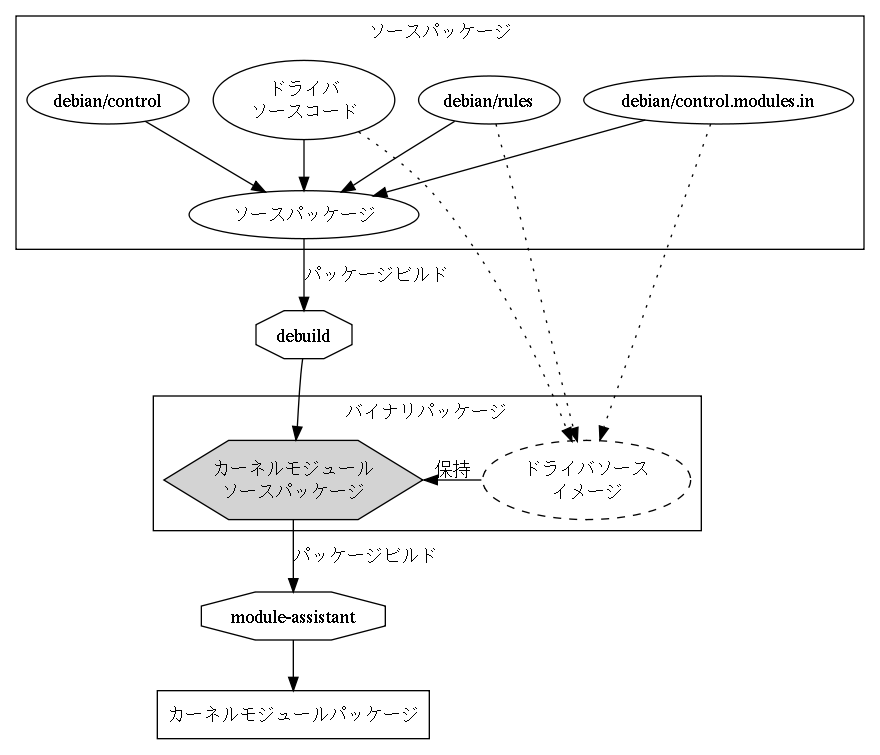
\includegraphics[width=0.8\hsize]{image200807/kmod0.png}
 \end{center}
 \caption{カーネルモジュールパッケージの仕組み}
 \label{fig:mod0}
\end{figure}

\subsection{ドライバソースコードの取得と展開}
vloopback は flashcam という フリーソフトウェアと共に提供されています。
今回は、vloopback のソースコードだけをターゲットにするので、ソースコードを
取り出します。
\begin{commandline}
$ wget http://www.swift-tools.net/Flashcam/flashcam-1.1.tgz
$ tar -xzf flashcam-1.1.tgz
$ cp -rf flashcam-1.1/vloopback-1.1.2 .
$ cd loopback-1.1.2
\end{commandline}

\subsection{dh\_make を使った雛形の作成}
パッケージ作成の準備ができたら、 dh\_make コマンドを使って雛形を作成します。
dh\_make には、カーネルモジュールの雛形を作成するオプション -k / --kmod が提供されています。

\begin{commandline}
$ dh_make -k -r 
Maintainer name : Nobuhiro Iwamatsu
Email-Address   : iwamatsu@nigauri.org 
Date            : Tue, 15 Jul 2008 23:21:23 +0900
Package Name    : vloopback
Version         : 1.1.2
License         : blank
Using dpatch    : no
Type of Package : Kernel Module
Hit <enter> to confirm: 
Done. Please edit the files in the debian/ subdirectory now. You should also
check that the vloopback Makefiles install into $DESTDIR and not in / .
\end{commandline}

\subsection{debianディレクトリ内の変更}
Debian パッケージにするための雛形が作成できたので、これを元に内容を変更していきます。

\subsubsection{サンプルスクリプト等の削除}
dh\_make で作成されるサンプルスクリプトは必要ないので全て削除します。
\begin{commandline}
$ rm -rf ./debian/*.ex ./debian/*.EX
\end{commandline}

\subsubsection{debian/copyright の修正}
パッチの情報に合わせて、debiab/copyright の修正を行います。
vloopback の場合は以下のように修正します。

\begin{commandline}
This package was debianized by Nobuhiro Iwamatsu <iwamatsu@nigauri.org> on
Tue, 15 Jul 2008 23:21:23 +0900.

It was downloaded from <http://www.swift-tools.net/Flashcam/flashcam-1.1.tgz>

Upstream Author(s):

    Olivier Debon <olivier@debon.net>

Copyright:

    Copyright (C) 2008 Olivier Debon <olivier@debon.net>

License:

    GPLv2

The Debian packaging is (C) 2008, Nobuhiro Iwamatsu <iwamatsu@nigauri.org> and
is licensed under the GPL, see `/usr/share/common-licenses/GPL'.

# Please also look if there are files or directories which have a
# different copyright/license attached and list them here.
\end{commandline}

\subsubsection{debian/README.Debian の修正}
debian/README.Debian ファイルを修正します。
雛形がある程度書いておいてくれているので、あまり修正する必要はありません。
確認した Linux カーネルバージョンなどを書いておくと良いかもしれません。

\begin{commandline}
vloopback for Debian
--------------------

Please see ./README for a description of the vloopback software.

The Debian vloopback source package provides two packages,

 vloopback-source, which provides the source for the kernel modules

The vloopback-source package can be used in several ways,

 - Using the make-kpkg(1) command provided by the kernel-package Debian
   package. This will produce a corresponding vloopback-modules package for
   the Debian kernel-image package that you are using. This is "the Debian
   way". See the "modules_image" section of the make-kpkg(1) man page.

 - Changing to the /usr/src/modules/vloopback/ directory and building as
   the README file instructs using "make; make install". This will build
   and install a module specific to the system you are building on and is
   not under control of the packaging system.

 -- Nobuhiro Iwamatsu <iwamatsu@nigauri.org>  Tue, 15 Jul 2008 23:21:23 +0900
\end{commandline}

\subsubsection{debian/control の修正}
次に debian/control ファイルを修正します。
dh\_make で作成した場合は、vloopback-utils といった、ドライバをサポートするための
パッケージを作成するエントリがあります。
ソースコードにツールが含まれている場合は、このエントリを使って、ツール用のパッケージを
作成できるようになっています。今回は必要ないので削除します。

\begin{commandline}
Source: vloopback
Section: graphics
Priority: extra
Maintainer: Nobuhiro Iwamatsu <iwamatsu@nigauri.org>
Build-Depends: debhelper (>= 7), bzip2
Standards-Version: 3.8.0.1
Homepage: http://www.swift-tools.net/Flashcam/

Package: vloopback-source
Architecture: all
Depends: module-assistant, debhelper (>= 7), make, bzip2
Description: Source for the vloopback driver.
 This package provides the source code for the vloopback kernel modules.
 The vloopback package is also required in order to make use of these
 modules. Kernel source or headers are required to compile these modules.
\end{commandline}

\subsubsection{debian/changelog の修正}
dch コマンドを使って debian/changelog ファイルを修正します。
\begin{commandline}
$ dch
vloopback (1.1.2-1) unstable; urgency=low

  * Initial release

 -- Nobuhiro Iwamatsu <iwamatsu@nigauri.org>  Tue, 15 Jul 2008 23:21:23 +0900
\end{commandline}

\subsubsection{control.modules.in ファイルの修正}
カーネルモジュールソースパッケージは 2つの control ファイルを持ちます。
一つは、カーネルモジュールソースパッケージ用、もう一つは カーネルモジュールパッケージ用の
カーネルモジュールソースパッケージ 用の debian/contorl ファイルが control.modules.in です。
ドライバパッケージ作成時に 
ソースパッケージからカーネルモジュールソースパッケージが作成され、ユーザはカーネルモジュールソースパッケージ
をコンパイルし、カーネルモジュールパッケージを作成し、インストールして利用します。
このファイルの中にはカーネルのバージョンによって置換される文字列が \texttt{\_KVERS\_} という文字列になっています。
{\bf control.modules.in} は {\bf module-assistant} などにより処理され、
各Linux カーネルバージョン用の内容に変更されます。

\begin{commandline}
Source: vloopback
Section: graphics
Priority: optional
Maintainer: Nobuhiro Iwamatsu <iwamatsu@nigauri.org>
Build-Depends: debhelper (>= 7)
Standards-Version: 3.8.0.1

Package: vloopback-modules-_KVERS_
Architecture: any
Provides: vloopback-modules
Description: vloopback modules for Linux (kernel _KVERS_).
 This package contains the set of loadable kernel modules for the
 <description>.
 .
 This package contains the compiled kernel modules for _KVERS_
 .
 If you have compiled your own kernel, you will most likely need to build
 your own vloopback-modules. The vloopback-source package has been
 provided for use with the Debian's module-assistant or kernel-package
 utilities to produce a version of vloopback-modules for your kernel.
\end{commandline}

\subsubsection{debian/rules ファイルの修正}

dh\_make で作成された、debian/rules ファイルは パッケージ作成用のターゲット(build/install/clean)と、
ドライバパッケージ作成用のターゲット binary-modules/kdist\_clean が用意されています。
これらのターゲットの中を修正します。
\begin{commandline}
#!/usr/bin/make -f

psource:=vloopback-source
sname:=vloopback

# prefix of the target package name
PACKAGE=vloopback-modules
# modifieable for experiments or debugging m-a
MA_DIR ?= /usr/share/modass
# load generic variable handling
-include $(MA_DIR)/include/generic.make
# load default rules, including kdist, kdist_image, ...
-include $(MA_DIR)/include/common-rules.make

kdist_config: prep-deb-files
kdist_clean: clean
	$(MAKE) $(MFLAGS) -f debian/rules clean

configure: configure-stamp
configure-stamp:
	dh_testdir
	# Add here commands to configure the package.

	touch configure-stamp

build-arch: configure-stamp  build-arch-stamp
build-arch-stamp: 
	dh_testdir

	# Add here command to compile/build the package.
	# $(MAKE)

	touch $@

#k = $(shell echo $(KVERS) | grep -q ^2.6 && echo k)

# during a normal build
binary-modules:
	dh_testroot
	dh_clean -k
	dh_installdirs lib/modules/$(KVERS)/misc

	# Build the module
	$(MAKE) KVER=$(KVERS) KSRC=$(KSRC)

	# Install the module
	cp vlooopbackko debian/$(PKGNAME)/lib/modules/$(KVERS)/misc

	dh_installdocs
	dh_installchangelogs
	dh_compress
	dh_fixperms
	dh_installdeb
	dh_gencontrol -- -v$(VERSION)
	dh_md5sums
	dh_builddeb --destdir=$(DEB_DESTDIR)
	dh_clean -k
\end{commandline}

\begin{commandline}
build-indep:  configure-stamp build-indep-stamp
build-indep-stamp: 
	dh_testdir
	touch $@

build: build-arch build-indep

clean: 
	dh_testdir
	rm -f build-arch-stamp build-indep-stamp configure-stamp
	dh_clean

install: DH_OPTIONS=
install: build
	dh_testdir
	dh_testroot
	dh_clean -k
	dh_installdirs

	# Create the directories to install the source into
	dh_installdirs -p$(psource)  usr/src/modules/$(sname)/debian

	# Copy only the driver source to the proper location
	cp vloopback.c  debian/$(psource)/usr/src/modules/$(sname)/.
	# Copy the needed debian/ pieces to the proper location
	cp debian/*modules.in* \
		debian/$(psource)/usr/src/modules/$(sname)/debian
	cp debian/rules debian/changelog debian/copyright \
		debian/compat debian/$(psource)/usr/src/modules/$(sname)/debian/
	cd debian/$(psource)/usr/src && tar c modules | bzip2 -9 > $(sname).tar.bz2 && rm -rf modules

	# Add here commands to install the package into debian/vloopback.
	# $(MAKE) DESTDIR=$(CURDIR)/debian/vloopback install

	dh_install

# Build architecture-independent files here.
# Pass -i to all debhelper commands in this target to reduce clutter.
binary-indep: build install
	dh_testdir -i
	dh_testroot -i
	dh_installchangelogs  -i
	dh_installdocs -i
	dh_installexamples -i
	dh_installman -i
	dh_link -i
	dh_compress -i
	dh_fixperms -i
	dh_installdeb -i
	dh_gencontrol -i
	dh_md5sums -i
	dh_builddeb -i

# Build architecture-dependent files here.
binary-arch: build install
	dh_testdir -s
	dh_testroot -s
	dh_installdocs -s
	dh_installinfo -s
	dh_installchangelogs  -s
	dh_compress -s
	dh_fixperms -s
	dh_installdeb -s
	dh_shlibdeps -s
	dh_gencontrol -s
	dh_md5sums -s
	dh_builddeb -s

binary: binary-indep binary-arch
.PHONY: build clean binary-indep binary-arch binary install configure binary-modules kdist kdist_configure kdist_image kdist_clean

\end{commandline}

\subsection{パッケージのビルドおよびインストール}
パッケージのビルドを行う際には、通常のパッケージ作成と変わりません。
debuild などを使ってパッケージの作成を行ってください。
作成されたパッケージをインストールすると、{\bf /usr/src/modules} にドライバソースイメージが
インストールされます。
\begin{commandline}
% debuild
% sudo dpkg -i ../vloopback-source_1.1.2-1_all.deb
\end{commandline}

\subsection{モジュールパッケージの作成}
\subsubsection{module-assistantを使ったコンパイル}
ドライバパッケージのコンパイルには module-assistant コマンドを利用します。
このコマンドは GUIを持っており、GUIでドライバのコンパイルやコンパイル環境の
アップデートを行う事ができます。
GUIで選択できるドライバ群は module-assistatパッケージ内で持っているリスト(/usr/share/modass/compliant.list)のみ
が対象になっているため、新しく作成したものは選択できません。
このような場合は、モジュール名を指定することによってコンパイル可能です。
\begin{commandline}
$ sudo m-a build vloopback
Extracting the package tarball, /usr/src/vloopback.tar.bz2, please wait...
/usr/bin/make clean
make[1]: ディレクトリ `/usr/src/modules/vloopback' に入ります

<snip>

make[3]: ディレクトリ `/usr/src/linux-headers-2.6.25-2-686' に入ります
  CC [M]  /usr/src/modules/vloopback/vloopback.o
  Building modules, stage 2.
  MODPOST 1 modules
  CC      /usr/src/modules/vloopback/vloopback.mod.o
  LD [M]  /usr/src/modules/vloopback/vloopback.ko
make[3]: ディレクトリ `/usr/src/linux-headers-2.6.25-2-686' から出ます
make[2]: ディレクトリ `/usr/src/modules/vloopback' から出ます
# Install the module
cp vloopback.ko debian/vloopback-modules-2.6.25-2-686/lib/modules/2.6.25-2-686/misc
dh_installdocs
dh_installchangelogs
dh_compress
dh_fixperms
dh_installdeb
dh_gencontrol -- -v1.1.2-1+2.6.25-6
dh_md5sums
dh_builddeb --destdir=/usr/src
dpkg-deb: `/usr/src/vloopback-modules-2.6.25-2-686_1.1.2-1+2.6.25-6_i386.deb' にパッケージ `vloopback-modules-2.6.25-2-686' を構築しています。
dh_clean -k

<snip>
\end{commandline}

\subsubsection{make-kpkgを使ったコンパイル}  
modules-assistant 以外にも make-kpkg の --added-modules オプションを使うことによって
コンパイルすることができます。しかし、make-kpkg の場合にはライバソースイメージを展開してくれない
ので、手動で展開する必要があります。
kernel-package はカーネルパッケージ専用と考えたほうがよさそうです。
(そのために modules-assistant ができたので。)

\subsection{まとめ}
今回は dh\_make からの作成でしたが、cdbs を使うともっと簡単かつ簡潔に作成することができます。
過去の勉強会資料にちょっとだけ載っているので、参考にしてください。
しかし、カーネルドライバ側の debian/rules は cdbs での対応が行われていないので、対応する
必要があるでしょう。
あと、最近はドライバも linus ツリーに取り込まれやすくなったのですが、
Linuxのリリース間隔などを考えると、新しいドライバは簡単に使えるものではありません。
新しいドライバを早く使いたい人には、ドライバパッケージ群が重要なパッケージになってくると思います。
そのためには、今後はこれらのパッケージをどのようにメンテナンスしていくかなどについて考えていく
必要がありそうです。

\subsection{おまけ}
module-assistant でサポートされているパッケージがどれぐらいコンパイルできるのか調べてみました。
アーキテクチャは i386 、ディストリビューションは sid です。パッケージは /usr/share/modass/compliant.list にかかれているものです。
結果は82個中、コンパイルOK: 22/ コンパイルNG: 22/ パッケージなし: 38 になりました。パッケージなしなのは、module-assistant のリストがメンテナンスされていなからだと思います。あとは、アーキテクチャ非対応など。
既にカーネルにマージされているものがけっこうあり、コンパイルエラーは各メンテナがサボっているのでしょう。
これらは今後BTSしていくつもりです。
 
\clearpage


%===========================================================%
\begin{getsureiupdate}{月例 Nexenta Operating System}{上川 純一}
\index{Nexenta}
先月につづいてNexentaをいじって見たのでお伝えします。

実用的なアプリケーションをビルドするまでに前回は至りませんでした。
そこで、今回はdlsym を使って自由自在にライブラリをロードできるようにしてみるところから
 まずやってみましょう。

dlsymでロードできる最低限の共有ライブラリを作成するところから始めてみま
しょう。


まず、関数一つだけを定義したCのファイルから最低限の共有ライブラリを作成
 してみ、それを実行するだけのプログラムと、dlopen経由で利用するプログラ
 ムを作成してみました。

\begin{commandline}
// a.c : サンプルの共有ライブラリのコード
#include <stdio.h>

void func1 (int i)
{
  printf(" hello world %i\n", i);
}
\end{commandline}

\begin{commandline}
// use.c: 通常の共有ライブラリ利用
#include <stdio.h>

void func1 (int i);

main()
{
  func1(1);
}
\end{commandline}

\begin{commandline}
// dlopen.c: dlopenでのバイナリ利用
#include <dlfcn.h>
static int (*myfunc1)(int i) = NULL;
int main()
{
  void* h=dlopen("./liba.so", RTLD_NOW);
  
  myfunc1=dlsym(h, "func1");
  
  myfunc1(10);
  
  return 0;
}
\end{commandline}

これらをコンパイル、リンクしてみて、動作を確認してみました。
どうやらLinuxとあまりかわらないようです。

\begin{commandline}
 + gcc -shared a.c -o liba.so
 + gcc use.c ./liba.so -o use
 + ./use
 hello world 1
 + gcc dlopen.c -o dlopen
 + ./dlopen
 hello world 10
\end{commandline}

ただし、これだけだとバージョンシンボルを利用した場合にdlsym ではどのバー
 ジョンを利用するのかが指定できないような雰囲気がただよっています。
というところまで確認したところで今月も力尽きました。
また来月続きをながめてみましょう。
もしかするとバージョンシンボルの作成とその利用をするかもしれません。

\end{getsureiupdate}
%===========================================================%


%\printindex

\cleartooddpage

\vspace*{15cm}
\hrule
\vspace{2mm}

\includegraphics[width=2cm]{image200502/openlogo-nd.eps}
\noindent \Large \bf Debian 勉強会資料\\ \\
\noindent \normalfont \debmtgyear{}年\debmtgmonth{}月\debmtgdate{}日 \hspace{5mm}  初版第1刷発行\\
\noindent \normalfont 東京エリア Debian 勉強会 (編集・印刷・発行)\\
\hrule


\end{document}
